\section{String Matching}
{\tiny find all occurrences of pattern p (length m) in text t (length n) \\
The size of the alphabet (q) is often an important factor\\
p occurs in t with shift s if p[0:m] == t[s:s+m]\\
A string x is a prefix/suffix of string y, if y=xw/ y=wx for a possibly empty string w\\}\\
\scriptsize{Brute-force string search}\\ 
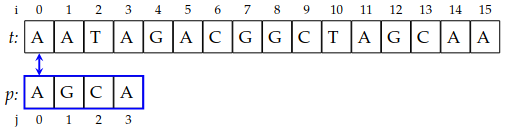
\includegraphics[scale=0.25]{string-match.png}\\{\tiny Start from the beginning, of i = 0 and j = 0\\
-if j == m, announce success with s = i\\
-if t[i]! = p[j]: shift p (increase i, set j = 0)\\
-otherwise: compare the next character (increase i and j, repeat)\\
worst case: t: AAAAAAAAC, p: AAC}\\
\scriptsize{Boyer-Moore algorithm}\\
{\tiny start comparing from the end of p\\
If t[i] does not occur in p, shift m steps\\
Otherwise, align the last occurrence of t[i] in p with t[i]\\
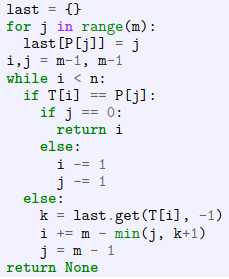
\includegraphics[scale=0.25]{boyer-moore.png}\\
on average performs better than brute-force\\
wost case complexity O(nm), e.g. t=aaaaaaa, p=baa\\
faster version exists O(n+m+q)
}\\
\scriptsize{FSA}\\
{\tiny 1. start at state 0, switch states based on the input\\
2. all unspecified transitions go to state 0\\
3. when at the accepting state, announce success\\
naive attemp building automaton O(qm**3)\\
matching O(n)\\
space requirement O(qm) if stored in matrix\\
faster algorithms for construction exists
}\\
\scriptsize{Knuth-Morris-Pratt (KMP) algorithm}\\ {\tiny 1. in case of a match, increment both i and j\\
2. on failure, or at the end of the pattern, decide which new p[j] compare with t[i] based on a function f\\
3. f[j-1] tells which j value to resume the comparisons from\\
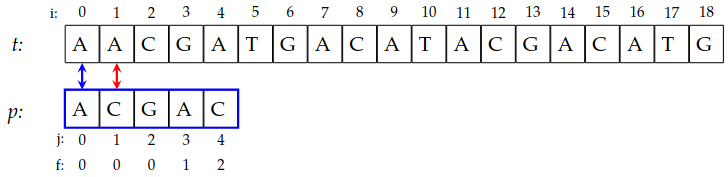
\includegraphics[scale=0.25]{kmp-demo.png}\\
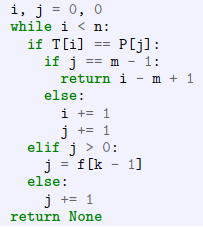
\includegraphics[scale=0.25]{kmp.png}\\
either increase i or shift the comparison\\
runs at most 2n times, complexity O(n)\\
build prefix/failure table\\
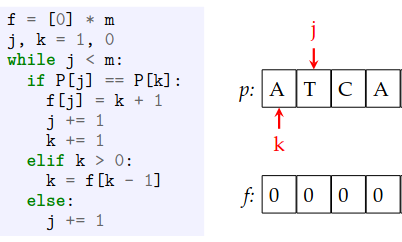
\includegraphics[scale=0.25]{failure-table.png}
}\\
\scriptsize{Robin-Karp algorithm}\\ {\tiny 1. instead of matching the string itself, matching the hash of it (based on a hash function)\\
2. If a match found, we need to verify – the match may be because of a hash collision\\
3. Otherwise, the algorithm makes a single comparison for each position in the text\\
a hash should be computed for each position (size m) (rolling hash functions avoid this complication)
}\\
\scriptsize{rolling hash function} {\tiny changes the hash value only based on the item coming in and going out of the window\\
to reduce collisions, better rolling-hash functions (e.g. polynomial hash functions) can be used
}